\documentclass[12pt]{article}
\usepackage{amsmath,amsthm,amssymb}
\usepackage{graphicx}
\usepackage{cite}
\pagestyle{myheadings}
\author{Joseph McDonald}

\textwidth=7in
\textheight= 9in

\topmargin=-0.5in
\oddsidemargin=-0.25in

\newcommand{\xbar}{\bar{x}}
\newcommand{\V}[1]{\boldsymbol{#1}}
\newcommand{\E}[0]{\mathbb{E}}
\title{Parallelizing AdaBoost and Decision Trees}

\begin{document}

%\begin{abstract}
%I present a parallelized construction of decision trees to be used in AdaBoost
%\end{abstract}

\maketitle

\begin{center}
Note that the source code and this paper are available at\\ {\tt https://github.com/josephpmcdonald/HPC15-ParallelBoosting/}
\end{center}

\section{Introduction}

\indent Binary and multiclass classification is a fundamental
problem in machine learning and is commonly one of the first concepts to be
studied in an introductory course. In the context of binary classification, a
labeled observation is a coordinate pair $(x, y)$ where $x\in\mathbb{R}^d$ is a
vector of data associated with the observation (feature vector) and $y\in\{1,
-1\}$ is the corresponding label of the observation. For example, $x_i$ might
be a point in $\mathbb{R}^2$ representing the height and weight of the $i$th
individual in a data set while the value of $y_i$ may indicate the individual's
gender. The goal in classification is to accurately predict the label
of a given observation using its feature vector. In this setting, the scenario
of supervised learning involves using a training set of labeled observations
$(x_i, y_i)$ to construct a prediction function $h$, one that takes a feature
vector $\hat{x}$ and gives a prediction on the corresponding label
$h(\hat{x})=\hat{y}$. To check the accuracy of the predictor it is common to use a separate set of test data, i.e. data that hasn't been used for training. There are many methods used to obtain a predictor for classification in supervised
learning, and the class of ensemble methods concerns combining several
predictors together.

Suppose now there exists an algorithm that, for any set of training data, is
guaranteed to give you a predictor that has at least 50\% accuracy. Such an
algorithm is called a weak learning algorithm since it yields a predictor that
performs marginally better than guessing randomly. The prediction functions
returned by a weak learning algorithm are called base classifiers, and a
natural question arises asking whether a combination of weak learners can be used
to make a strong learner, or one that can achieve a certain level of accuracy.
Ensemble methods like this are called boosting, and the
algorithm AdaBoost introduced in \cite{FS} accomplishes this through
successive rounds of training a weak learner to the data and subsequently
re-weighting the training samples \cite{FS}.

The goal of this project is to implement a parallelized version of decision trees, a commonly
used weak learner, in order to improve the running time of AdaBoost. We
give a short overview of AdaBoost and decision trees in the next section,
describe the implementation of the decision trees, the data sets used and the
results comparing the serial and parallelized execution of the boosting algorithm. 

\section{AdaBoost}

\indent The beauty of AdaBoost is in using a relatively inaccurate
weak learning algorithm to produce a much more accurate prediction function. In
each round of AdaBoost for $t$ from 1 to $T$, the weak learner selects a
base classifier $h_t: \mathbb{R}^n\rightarrow\{1,-1\}$ from a set of functions
$H$, in particular choosing the one with the least error
$\epsilon_t=\sum_{i=1}^{n}D_t(i)I(h_t(x_i)\neq y_i)$ (Line 4), where $D_t(i)$ is
the weight associated with the $i$th sample. The coefficients $\alpha_t$ and $Z_t$ are calculated, where $\alpha_t$ is used in the ensemble prediction function and $Z_t$ is a normalization constant. The algorithm then updates the
weights in Line 8 to place more emphasis on the samples that $h_t$ misclassified,
so that in future rounds the base classifiers are chosen to correct these mistakes. The predictor that is
returned in Line 9 after $T$ rounds is a linear combination of all $h_t$'s. Note the
coefficient $\alpha_t$ gives more weight in the final predictor to the classifiers from rounds that fared better.
We give the algorithm as detailed in \cite{Mohri} below.\\ \\
{\sc AdaBoost}: $S = \{(x_i,y_i):i = 1\ldots n\}$
\begin{enumerate}
\itemsep1pt \parskip0pt \parsep0pt
\item {\bf for $i=1$ to $n$}
\item \quad $D_1(i) = \frac{1}{n}$
\item {\bf for $t=1$ to $T$}
\item \quad $h_t$ = {\sc WeakLearner}$(S\sim D_t)$ with weighted error $\epsilon_t$
\item \quad $\alpha_t = \frac{1}{2}\log(\frac{1-\epsilon_t}{\epsilon_t})$
\item \quad $Z_t = 2[\epsilon_t(1-\epsilon_t)]^{1/2}$ (normalization factor)
\item \quad {\bf for $i = 1$ to $n$}
\item \quad \quad $D_{t+1}(i) = \frac{D_t(i)\exp(-\alpha_t y_i h_t(x_i))}{Z_t}$
\item $g = \sum_{t=1}^T \alpha_t h_t$
\item {\bf return} $\mbox{sign}(g)$
\end{enumerate}

Note that everything except Line 4 can be done relatively quickly, so improving
the speed of the weak learning algorithm will improve the speed of AdaBoost by
a similar factor. 

\section{Decision Trees}

\indent Decision trees are a well-known method used in classification which
partitions the feature space into rectangular regions and applies to each
region the most frequent label among the training set points it contains. In
the most common decision tree algorithms each partition of the feature space is
made along coordinate axes and is done in a heirarchical way. Initially, a line
parallel to an axis divides the space into two regions, and then the same is
done for these resulting regions. This process is repeated many times until the
space is partitioned into several rectangles, like the example in Figure 1, taken from
\cite{HTF}. Each split is made to separate points of the two distinct classes
into different regions as best as possible. Thus the two resulting rectangles
will have less {\it impurity} in comparison to the parent node.


There are a few common ways to measure impurity for a given region containing
sample points. Gini index is used here which can be easily substituted for
others. For two classes the Gini Index of region $A$ is $I(A) = 2p(1-p)$ where
$p$ is the probability of choosing a point in the first class from $A$, which
translates to the probability of incorrectly guessing the class of a randomly
chosen point from either class.

The splitting of regions gives rise to the tree structure. At each node in the
tree, the samples in the region corresponding to that node are ordered and
counted to find in which dimension that region can be divided that gives the
greatest decrease in the impurity of the branch. Figure 2 shows an example of
this where at the top of the tree the decision to split on the first feature
$X_1$ is best and the separation is made at $t_1$. In the first of the two
resulting regions it is determined that the best split is made on $X_2$ at
$t_2$, and in the other region the best separation is on $X_1$ at $t_3$. This
splitting process will go on until a stopping criterion is met, either if there
are too few sample points in a region or if no gain in purity can be made by
splitting on any feature.

%In Figure 1, the lines drawn at $t_i$ represent the division of the previous
%region. Since each region is divided in two until a stopping criterion is met,
%this gives rise to a binary tree where the action at each node is a line that
%partitioning the region at that node. At each level of the tree the tree
%corresponding to Figure 1 is given in Figure 2 (\cite{HTF}). As depicted in the
%two figures, the splitting of each node is done in a heirarchical way so that .
%The feature space is partitioned along coordinate axes, which gives rise to
%decision. The most common way to partition the feature space is along
%coordinate axes. 

\begin{figure}[h!]
\centering
\begin{minipage}{0.45\textwidth}
\centering
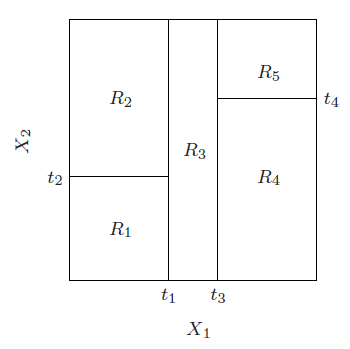
\includegraphics[width=2.5in]{partition}
\caption{space partitioned by a decision tree, from \cite{HTF}}
\end{minipage}\hfill
\begin{minipage}{0.45\textwidth}
\centering
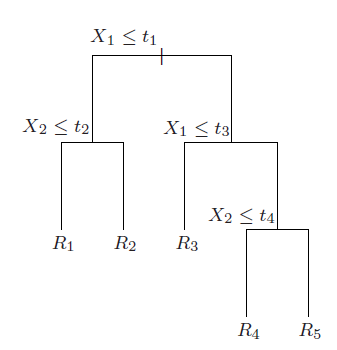
\includegraphics[width=2.5in]{dectree}
\caption{decision tree structure, from \cite{HTF}}
\end{minipage}
\end{figure}

\section{Implementation}


Since the tree-building process is the most time-consuming portion of AdaBoost,
our goal is to parallelize this. It seems natural to divide amongst processors
the work of finding the dimension in the feature space that best splits the
region and increases the purity for each node in the tree. The datasets we are
handling have several dimensions, on the order of tens to hundreds, so each
processor could be responsible for a group of dimensions in the feature space.

The AdaBoost algorithm is written in the main method of the program contained
in {\tt paraboost.c}. This file also contains a few methods for utility, one
that converts a decision tree data structure into a useable function and
another that calculates weighted error. main() also performs load balancing by
determing the features that each processor is responsible for. 

The methods that collect data from files on the hard disk and organize storage
are defined in {\tt data.c}. These methods scrape floats from text and binary
files and allocate space on the heap to store feature vectors and their labels.
main() calls them early to load the training data in memory. There are a number
of different sorting routines in {\tt sort.c}, all implementations of QuickSort
or MergeSort that vary with the structure of the data types they sort. These
methods are used to order data structures prior to the decision tree
construction.

The methods that implement decision tree operations are located in {\tt
tree.c}. ParallelSplit() performs the parallel node splitting procedure for a
given node in a decision tree, using the data points in that node to find the
partition minimizing the impurity of the resulting child nodes. It calls the
subroutine PodWBS() for each feature, which computes the impurity for every
possible partition of the data over that feature dimension and returns an index
corresponding to the best partition for that dimension and the impurity. Since
this is done for every feature the processor is responsible for,
ParallelSplit() then broadcasts which of its features is best and the minimum
impurity to every processor. Thus an Allreduce is performed in order to
determine which feature among all has the best partition achieving the minimum
impurity. This determines the two branches of the decision tree, and the root
processor informs the others which branch of the tree each observation goes to.
The arrays of pointers to these observations are re-sorted to reflect this and
ParallelSplit() is then called recursively on each of the two child nodes.
After an end condition is met (depth in tree, small number of points
in node, or very low impurity) the function returns. This method is called for every node in the tree and performs noticeable computation for all nodes that aren't leaves.


%After each processor determines the best dimension to split on amongst those
%it's responsible for, we can perform a reduction and determine the best split
%over all dimensions. 


Any tree will split the feature space multiple times so
there are several occasions for parallelism to speed up execution. In testing I
commonly set the maximum depth for a tree to between two to five levels. Also
the number of rounds of AdaBoost, and hence the number of trees constructed, is
a parameter in the method allowing you to affect how often the algorithm executes in parallel.




\section{Data and Timings}
We employ the MNIST dataset \cite{MNIST} to test our implementation. MNIST is a collection of 70,000 images of handwritten digits commonly used in image processing and pattern recognition research. The grayscale images are written in a binary file and consist of 28x28 arrays of integers ranging from 0 to 255 representing pixels varying from white to black. From this we separate out the set of 1's and 7's with the goal of performing binary classification between these two digits. It's common to also try this with the digits 4 and 9. This dataset can be obtained from \cite{MNIST}, and they are the four files referred to as the training set and test set images and labels, where the training set images and labels are called {\tt train-images-idx3-ubyte} and {\tt train-labels-idx3-ubyte} respectively. There are roughly 13,000 instances of 1's and 7's among the training set.

To test the parallel efficiency of this implementation, I ran the program on the host {\bf crunchy1} with 20 rounds of boosting with varying the number of processors as given in the following table. This gives the amount of time it took for the program to run as a whole in addition to the average time per processor spent constructing trees, since I wanted to measure the time spent in parallel without the extra overhead time performing serial tasks.

\begin{center}
\begin{tabular}{|r|r|r|r|r|r|}
\hline
no. of processors &1&2&4&8&16\\ \hline
elapsed time (s) &56.72 &25.88 &12.94 &6.52 &3.03 \\ \hline
avg. tree-building time (s) &36.898 &16.825 &8.632 &4.434 &1.915 \\ \hline
\end{tabular}
\end{center}

A noticeable speedup occurs, and doubling the number of processors roughly splits the time in half at each stage. This was done on a cluster with four 16-core processors so we aren't hitting any performance walls. However when attempting this on my local machine with eight cores, while it performed the computations faster I did not see the same gains in doubling the number of processors. There were less improvements in going from one processor to two to four, though they were still noticeable. And using all eight took more time than just four, though perhaps that ought to be expected since there are other processes going on in the background. Nevertheless, using the {\bf crunchy1} host showed the improvements gained by utilizing a parallel structure for building the decision trees.



\section{Useage}
I used MPICH for the MPI processor communications. To use the parallel boosting tool, include the file {\tt makefile} in the folder with the source code and compile it to create the executable {\tt pboost}. Using the command {\tt mpirun}, specify the number of processors and list the number of boosting rounds to perform after the executable. For instance, to run the executable with four processors for 50 rounds:

\begin{center}
{\tt mpirun -np 4 ./pboost 50}
\end{center}

\noindent The source code and this paper are available at:
\begin{center}
{\tt https://github.com/josephpmcdonald/HPC15-ParallelBoosting/}
\end{center}

%\maketitle
%
%\section{Introduction}
%Binary and multiclass classification is a fundamental problem in machine
%learning and is commonly one of the first concepts to be studied in an
%introductory course, the goal being to accurately predict the label of a given
%observations using the data associated with the observation. In the context of
%binary classification, a labeled observation (or sample point) is a coordinate
%pair $(x, y)$ where $x\in\mathbb{R}^d$ is a vector of data associated with the
%observation (feature vector) and $y\in\{1, -1\}$ is the corresponding label of
%the observation. This classification, and even prediction in general, commonly
%splits up into two different scenarios, supervised and unsupervised learning.
%Supervised learning involves taking a set of labeled observations (training
%set) and using it to construct a prediction function, one that can take a new
%feature vector and predict the corresponding label. There are many methods used
%for classification in supervised learning, including support vector machines,
%decision trees, online algorithms, and many others.
%
%A weak learning algorithm, or weak learner, is an algorithm that, given a set of training data, yields a predictor with performance of at least 50\% percent accuracy, or just better than random guessing. The prediction functions that a weak learner returns are called base classifiers. There was an important question asking whether the base classifiers from a weak learner could somehow be joined together to produce a strong learner, or an algorithm that gives a prediction function of arbitrary accuracy.
%
%Boosting is a category of methods that addresses this question, which Freund and Schapire
%successfully answered with their algorithm AdaBoost. AdaBoost, which stands for adaptive boosting, builds
%a more accurate predictor through successive rounds of training a weak learner
%to the data and subsequently re-weighting the training samples \cite{no1}. 




\begin{thebibliography}{99}
\bibitem{FS} Yoav Freund and Rob Schapire. A Decision-Theoretic Generalization of On-Line Learning
and an Application to Boosting. {\it Journal of Computer and System Sciences}, 55:119-139, 1997.
\bibitem{HTF} T. Hastie, R. Tibshirani, J. Friedman. {\it The Elements of Statistical Learning: Data Mining, Inference, and Prediction}. Springer-Verlag, 2009.
\bibitem{Mohri} M. Mohri, A. Rostamizadeh, A. Talwalkar. {\it Foundations of Machine Learning}. MIT press, 2012.
\bibitem{no4} "AdaBoost". {\it Wikipedia}. {\tt https://en.wikipedia.org/wiki/AdaBoost}
\bibitem{MNIST} Yann LeCun, Corinna Cortes, Christopher J. C. Burges. {\it The MNIST Database}. {\tt http://yann.lecun.com/exdb/mnist/}
\end{thebibliography}
\end{document}



